\section{Raft}
As of writing this report, the most recent proposal to solving the consensus problem is Raft \cite{Raft}. Diego Ongaro and John Oustershout argue that most consensus algorithms, such as Paxos \cite{Paxos} suffer from poor understandability and are hard to teach and later implement. They then introduce Raft as a simple and understandable solution to the consensus problem. They describe Raft as three main components:
\begin{itemize}
\item \textbf{Leader election}: A strong leader is elected which responsible for keeping the rest of the system in consensus for a term, that ends if it fails.
\item \textbf{Log replication}: The leader must accept log entries from clients and replicate them across the cluster, forcing the other logs to agree with its own.\cite{Raft}. The leader must also update the logs of other servers if they are not up to date.
\item \textbf{Safety}: The specified design provides safety such that\cite{Raft}: 
    \begin{itemize}
    \item \textbf{Election Safety}: There is always is at most one leader in the system.
    \item \textbf{Leader Append-Only}: A leader only appends new entries to its log i.e. doesn't overwrite existing entries.
    \item \textbf{Log Matching}: All logs of all servers are matching up to their latest common index.
    \item \textbf{Leader Completeness}: No newly elected leaders will overwrite other servers logs if its own log entry is not up to date.
    \item \textbf{State Machine Safety}: When a server updates its log it must be up to date with the leaders log.
    \end{itemize}
\end{itemize}
So the basis of this solution is the leader election after which the given leader is responsible to replicate commands it receives from a client to the rest of the network. All servers contain an implementation of Raft, having a log of entries pushed by a client.A server can be in three states: leader, candidate or follower. Figure \ref{fig:election_example} illustrated the scenario in which a leader is elected. At initial system start up every server is a follower until $P1$ times out and becomes a candidate. If this candidate receives a majority vote, it then transitions to the leader state after which it has the responsibilities described above. This leader then maintains log matching by continuously sending empty messages i.e. heart beats in order to update servers with logs that are not up to date. \\ \\
Figure \ref{fig:failure_example} then shows how Raft will tolerate a faulty leader. Here we see that the leader $P1$ fails by crashing. $P4$ then times outs and initiates a new election.

\begin{figure}[ht]
\centering
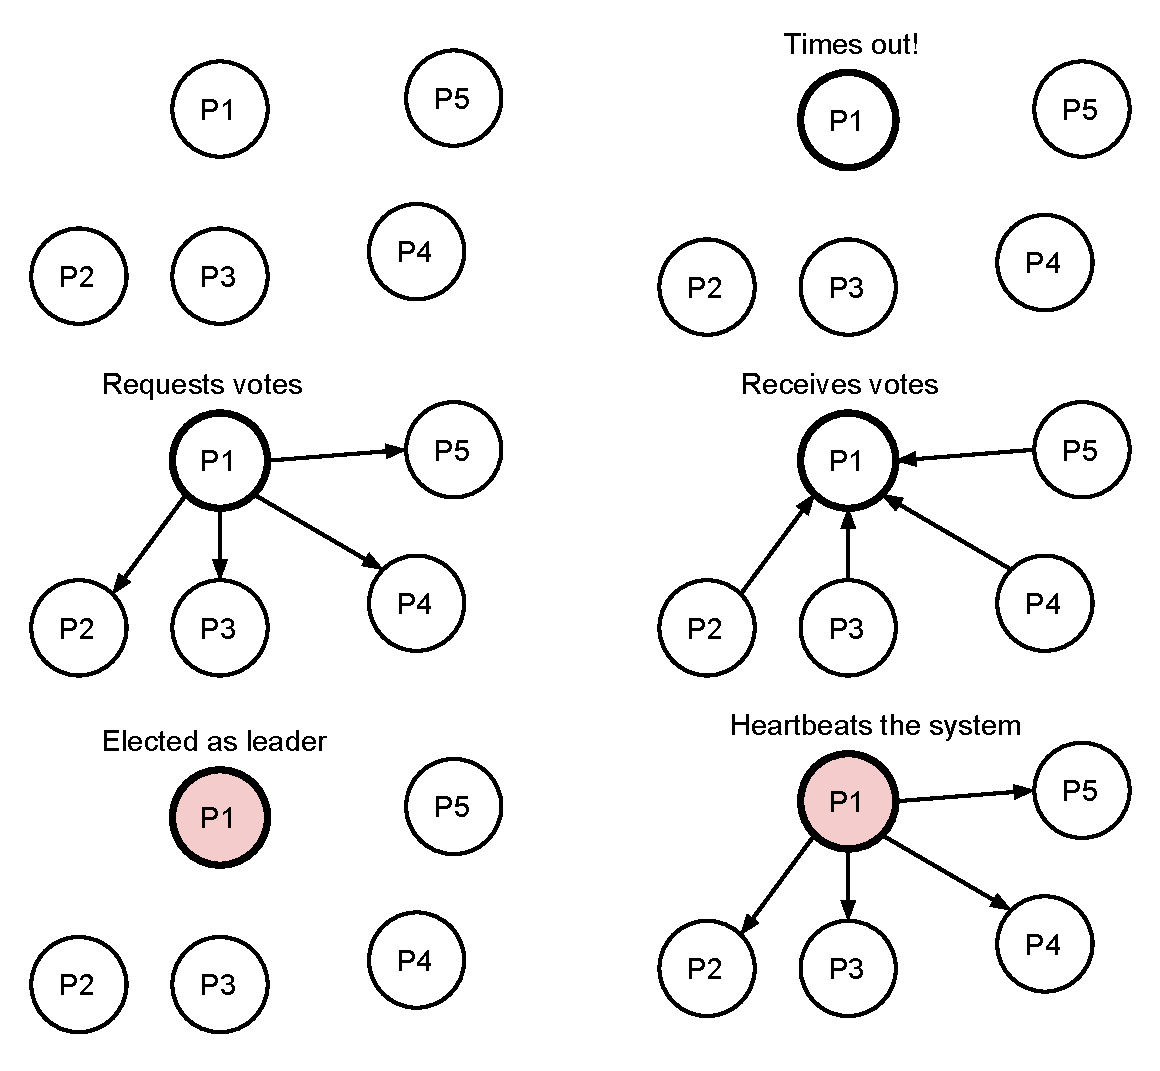
\includegraphics[scale = 0.35]{election-example}
\caption{A simple scenario where 5 servers are to obtain consensus by first electing a leader.}
\label{fig:election_example}
\end{figure}

\begin{figure}[ht]
\centering
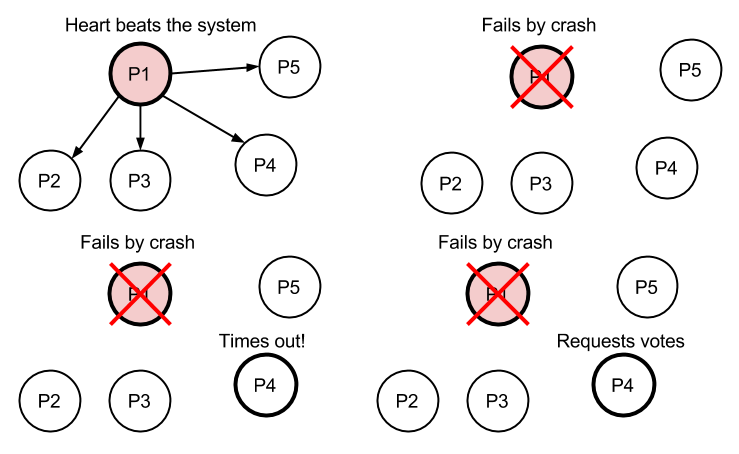
\includegraphics[scale = 0.35]{failure-example}
\caption{A simple scenario where a leader $P1$ crashes after which $P4$ times out and start a new election.}
\label{fig:failure_example}
\end{figure}

It should also be noted that, since the availability provided by Raft relies on majority votes and non-Byzantine failures only i.e. failure is a server stopping and not giving sending incorrect messages, the algorithm can only uphold these properties in a network where $3F \leq N$, where $F$ is the amount of failures and $N$ is the amount of processes in the system.
\\ \\
Looking back at the Two Generals Problem, Raft would only be able to solve the problem if a majority vote would be possible, which it is not. So in order to solve this problem when utilising Raft, one must add another general - such that there is now three generals instead of two. We should also modify the problem, such that the messenger always tells the truth (i.e. cannot suffer from Byzantine failure). So now that we have three generals and an 'uncapturable' messenger, they will reach consensus by finding a leader after which he decides when to launch the attack.
\\ \\
The above description of Raft serves as a rough overview of the algorithm. A more detailed description will be given during the implementation since the paper has implicit or unclear implementation specific components that we have to figure out ourselves. So as we every component is describes our experiences and findings in terms of implementation specific choices will thus be documented.